% [原文 p.39]
那么，先来证明最初的丰富性判别法。

\begin{theoremp}[{中井--Moishezon 判别法}]{1.37}
设 $X$ 为域上的固有概形，$L$ 为 $X$ 上的 Cartier 除子。此时，$L$ 在 $X$ 上丰富的充要条件是
\[ (L^{\dim Z}\cdot Z)>0 \]
对一切闭子概形 $Z\subset X$ 成立。
\end{theoremp}

\begin{proof}
只对 $X$ 射影的情形证明定理。

若 $L$ 丰富，则可设 $X\subset\PP^N$ 且 $\cO_X(mL)=\cO_X(1)$。此时 $m^d(L^d\cdot Z)=\deg Z>0$（命题 1.35(3)）。

为证明逆命题，使用 Noether 式归纳法。于是可设对一切闭子概形 $Z\subsetneq X$，$L|_Z$ 丰富。进一步可设 $n=\dim X>0$。

\textbf{步骤 1}\quad 存在 $k>0$ 使 $h^0(X,\cO_X(kL))>0$。

设 $B$ 是 $X$ 上十分丰富的有效 Cartier 除子，且 $L+B$ 也十分丰富。此时，一般元 $A\in|L+B|$ 是有效 Cartier 除子，且 $L\sim A-B$ 成立。在正合列
\[ 0\to\cO_X(kL-B)\to\cO_X(kL)\to\cO_B(kL)\to0 \]
中，$\cO_B(L)$ 由归纳法丰富。特别地，$k\gg0$、$i\ge1$ 时 $h^i(B,\cO_B(kL))=0$，故 $k\gg0$、$i\ge2$ 时 $h^i(X,\cO_X(kL-B))=h^i(X,\cO_X(kL))$。又由正合列
\[ 0\to\cO_X(kL-B)\to\cO_X((k+1)L)\to\cO_A((k+1)L)\to0 \]
同样得到等式 $h^i(X,\cO_X(kL-B))=h^i(X,\cO_X((k+1)L))$（$k\gg0$，$i\ge2$）。以上可知 $h^i(X,\cO_X((k+1)L))=h^i(X,\cO_X(kL))$，即 $i\ge2$ 时 $h^i(X,\cO_X(kL))$ 在 $k\gg0$ 时为常数。于是
\begin{align*}
h^0(X,\cO_X(kL))&\ge h^0(X,\cO_X(kL))-h^1(X,\cO_X(kL))\\
&=\chi(X,\cO_X(kL))+(\text{常数})\\
&=(L^n)/n!\cdot k^n+(\text{更低次项之和}).
\end{align*}

\textbf{步骤 2}\quad 存在 $k>0$ 使 $\cO_X(kL)$ 由全局截面生成。

% [原文 p.40]
由步骤 1，存在 $m>0$ 与非零元 $s\in H^0(X,\cO_X(mL))$。定义 $D:=(s=0)\subset X$，则对 $X$ 的某个闭子概形 $Y$ 有
\[ \cO_Y\cong\operatorname{im}[\cO_X\xrightarrow{s}\cO_X(mL)]=\ker[\cO_X(mL)\to\cO_D(mL)]. \]
注意：$s$ 可能在 $X$ 的某个成分上处处为 $0$，故 $Y\ne X$ 也可能发生。有正合列
\[ 0\to\cO_Y((k-1)mL)\to\cO_X(kmL)\to\cO_D(kmL)\to0. \]
$k\gg0$ 时 $\cO_D(kmL)$ 十分丰富，故只需证明 $k\gg0$ 时
\[ H^0(X,\cO_X(kmL))\to H^0(D,\cO_D(kmL)) \]
满射即可。

若 $Y\subsetneq X$，则由归纳法，$k\gg0$ 时 $H^1(Y,\cO_Y(kmL))=0$，从而得到满射。故可设 $Y=X$，即 $D$ 是 Cartier 除子。由归纳法，$k\gg0$ 时 $H^1(D,\cO_D(kmL))=0$。与步骤 1 同样可知 $k\gg0$ 时 $h^1(X,\cO_X(kD))$ 是 $k$ 的非增函数。由此可知 $k\gg0$ 时 $H^0(X,\cO_X(kmL))\to H^0(D,\cO_D(kmL))$ 满射。

\textbf{步骤 3}\quad 对适当的 $k>0$，设 $\phi:X\to\PP^N$ 为由 $|kL|$ 决定的态射。此时 $\phi$ 是有限态射。事实上，若曲线 $C\subset X$ 使 $\phi(C)$ 成为点，则 $\cO_X(kL)|_C\cong\cO_C$，由命题 1.35(1) 与命题 1.35(4) 得 $(L\cdot C)=0$。
\end{proof}

% [Tutor Note: 步骤 1 最后那串不等式的第一行在原书页图上写作 $h^0\ge h^0-h^1$，本身是平凡的；真正的信息在第二、三行：$h^i$（$i\ge2$）为常数，故 $h^0$ 随 $k^n$ 增长。照原文翻译，勿擅自“修正”。]

下面还需要 [Kle66] 关于 nef 除子的下列性质。

\begin{theoremp}{1.38}
设 $X$ 为固有簇，$L$ 为 nef Cartier 除子。此时，对任意闭子概形 $Z\subset X$ 有 $(L^{\dim Z}\cdot Z)\ge0$。
\end{theoremp}

\begin{proof}
只对射影的 $X$ 证明。一般情形由 Chow 引理与命题 1.35(6) 容易归结为射影情形。

设 $n=\dim X$。对 $n$ 作归纳法证明 $(L^{\dim Z}\cdot Z)\ge0$。若 $Z\subsetneq X$，则由归纳法假设得 $(L^{\dim Z}\cdot Z)\ge0$。故只需证明 $(L^n)\ge0$。

% [原文 p.41]
设 $A$ 是 $X$ 上十分丰富的除子，令
\[ f(x,y):=((xL+yA)^n)=\sum_{i=0}^n\binom{n}{i}(L^{n-i}\cdot A^i)x^{n-i}y^i. \]
这是关于 $x$、$y$ 的 $n$ 次齐次多项式。选取一般元 $A_j\in|A|$。此时由命题 1.35(5) 有 $(L^{n-i}\cdot A^i)=(L^{n-i}\cdot(A_1\cap\cdots\cap A_i))$，故由归纳法，$(L^{n-i}\cdot A^i)\ge0$ 对 $i=1,\dots,n-1$ 成立。又由命题 1.35(3) 有 $(A^n)>0$。

$f(1,t)$ 的系数除常数项外全都非负。因此 $f(1,t)$ 是 $t\ge0$ 上的严格增函数。若 $f(1,0)=(L^n)<0$，则恰好存在一个正数 $t_0>0$ 使 $f(1,t_0)=0$。由这一假设导出矛盾。
\begin{equation}\tag{1.5}
0=f(1,t_0)=((L+t_0A)^n)=(L\cdot(L+t_0A)^{n-1})+t_0(A\cdot(L+t_0A)^{n-1}).
\end{equation}
为估计右端第 $1$ 项，取有理数 $s=a/b>t_0$，其中 $a,b\in\Z_{>0}$。此时 $((bL+aA)^n)=b^nf(1,s)>0$；且对 $Z\subset X$，
\begin{equation}\tag{1.6}
\begin{aligned}
((bL+aA)^d\cdot Z)&=\sum_{i=0}^d\binom{d}{i}(L^{d-i}\cdot A^i\cdot Z)b^{d-i}a^i\\
&\ge(A^d\cdot Z)a^d>0
\end{aligned}
\end{equation}
由归纳法成立。因此 $bL+aA$ 由定理 1.37 是丰富的。

$m\gg0$ 时，存在与 $m(bL+aA)$ 横截相交的元 $H_1,\dots,H_{n-1}$。此时由命题 1.35(5)，
\[ m^{n-1}(L\cdot(bL+aA)^{n-1})=(L\cdot H_1\cap\cdots\cap H_{n-1})\ge0. \]
因此
\[ (L\cdot(L+t_0A)^{n-1})=\lim_{s\to t_0}(L\cdot(L+sA)^{n-1})\ge0. \]
由 $Z=A$ 时的不等式 (1.6) 得 $(A\cdot(L+t_0A)^{n-1})\ge t_0^{n-1}(A^n)>0$。把它代入等式 (1.5) 便得矛盾。
\end{proof}

% [Tutor Note: 这段证明的关键是 $f(1,t)$ 的系数非负，于是 $f(1,t)$ 严格增；再把 $s>t_0$ 的“丰富性”通过 (1.6) 与极限传回 $t_0$，负的 $(L^n)$ 就无处可逃。]

\par\medskip\noindent\textbf{1.39}（Kleiman 丰富性判别法（定理 1.18）的证明）\quad 设 $D$ 丰富。则可把它取为 $N_1(X)^*\otimes\Q$ 的基底 $D=D_1,\dots,D_{\rho(X)}$ 的一部分。进一步可设 $D_i$ 与 $2D-D_i$ 都是丰富的 $\Q$-除子。此时，由 $n(C):=\sum_i|(C\cdot D_i)|$ 定义的 $n:N_1(X)\to\R$ 是 $N_1(X)$ 的范数。对一切 $C\in\overline{NE}(X)\setminus\{0\}$ 有
% [原文 p.42]
$2\rho(X)(C\cdot D)-n(C)=(C\cdot\sum(2D-D_i))\ge0$，故得 $(C\cdot D)\ge n(C)/(2\rho(X))>0$。

为看逆命题，设 $A$ 是 $X$ 的丰富除子。$D$ 在 $\overline{NE}(X)\setminus\{0\}$ 上真正为正（$>0$）。因此 $L:=tD-A$ 对某个整数 $t\gg0$ 成为 nef。由定理 1.38，对一切 $Z\subset X$，$tD=A+L$ 满足
\[ t^{\dim Z}(D^{\dim Z}\cdot Z)\ge(A^{\dim Z}\cdot Z)>0. \]
于是 $tD$ 由定理 1.37 丰富。\hfill$\blacksquare$

\begin{remark}{1.40}
当 $X$ 固有且非奇异（或至少是 $\Q$-分解的）时定理 1.18 也成立，但对一切固有簇并不成立。详情请参看 [Kle66, Har70, Kol96]。
\end{remark}

% [Tutor Note: 判别法有两个方向：由丰富推锥上的正性（用 $D_i$ 与 $2D-D_i$ 造范数），再由正性经定理 1.38 与定理 1.37 推回丰富。后者用到 $tD$ 对一切 $Z$ 的交点数为正，正是把“锥上为正”翻译成“逐个子概形为正”的桥梁。]

若使用下一命题，则上述结果可推广到相对的情形。

\begin{propositionp}{1.41}
设 $f:X\to Y$ 为固有态射，$D$ 是 $X$ 上的 Cartier 除子，取一点 $y\in Y$，$X_y$ 是 $f$ 在 $y$ 上的纤维。若 $\cO_{X_y}(D)$ 丰富，则 $D$ 在 $Y$ 的某个开集 $U\ni y$ 上丰富。
\end{propositionp}

\begin{proof}
作为第 $1$ 阶段，先证明下列消没定理。

（$*$）对 $f^{-1}(y)$ 的近旁定义了的任意凝聚层 $F$，$i>0$、$\nu\gg0$ 时 $R^if_*F(\nu D)=0$ 在 $y$ 的近旁成立。

（$*$）的证明用关于 $i$ 的降链归纳法。消没定理在 $i>\dim f^{-1}(y)$ 时已知，故可对某个 $i>1$ 假设（$*$）。设 $u_1,\dots,u_r$ 是极大理想 $m_{y,Y}$ 的生成元，$s:F^{\oplus r}\to F$ 是 $f^{-1}(y)$ 近旁定义的同态 $s(a_1,\dots,a_r):=\sum_i u_ia_i$。此时得到正合列
\[ F(\nu D)^{\oplus r}\xrightarrow{s(\nu D)}F(\nu D)\to\cO_{X_y}\otimes F(\nu D)\to0. \]
由 $D|_{X_y}$ 的丰富性与归纳法假设 $R^if_*(\ker s)(\nu D)=0$，可知 $\nu\gg0$ 时在 $y$ 的近旁有正合列
\[ R^{i-1}f_*(\operatorname{im}s)(\nu D)\to R^{i-1}f_*F(\nu D)\to R^{i-1}(f_y)_*(\cO_{X_y}\otimes F)(\nu D)=0, \]
% [原文 p.43]
\[ R^{i-1}f_*F(\nu D)^{\oplus r}\to R^{i-1}f_*(\operatorname{im}s)(\nu D)\to R^if_*(\ker s)(\nu D)=0. \]
组合这些便得正合列
\[ R^{i-1}f_*F(\nu D)^{\oplus r}\to R^{i-1}f_*F(\nu D)\to0. \]
故 $R^{i-1}f_*F(\nu D)=m_{y,Y}R^{i-1}f_*F(\nu D)$，由中山引理得 $R^{i-1}f_*F(\nu D)=0$。于是消没定理对 $i-1$ 成立，（$*$）得证。

设 $I$ 是 $X_y$ 的定义理想层。对 $I$ 应用（$*$），便得 $\nu\gg1$ 时 $f_*\cO_X(\nu D)\to\cO_{X_y}(\nu D)$。由于 $\cO_{X_y}(D)$ 丰富，$\nu\gg1$ 时 $\cO_{X_y}(\nu D)$ 由全局截面生成。因此合成
\[ f^*f_*\cO_X(\nu D)\to\cO_X(\nu D)\to\cO_{X_y}(\nu D) \]
在 $\nu\gg1$ 时满射。由中山引理，$f^*f_*\cO_X(\nu D)\to\cO_X(\nu D)$ 在 $Y$ 的仿射开集 $U\ni y$ 上为满射，且 $\nu D|_{f^{-1}(U)}$ 在 $f^{-1}(y)$ 的近旁定义有限态射。至此命题 1.41 证毕。
\end{proof}

% [Tutor Note: 这一证明是“相对化”的标准套路：先把消没定理沿纤维方向作归纳，再用中山引理把“逐点可生成”提升为“邻域上可生成”。注意 $f^{-1}(y)$ 只是纤维的近旁，并非整个 $X$。]

% [原文 p.44]
下面是中井--Moishezon 判别法的相对版，用命题 1.41 即可由定理 1.37 立即得到。

\begin{theorem}[{相对的中井--Moishezon 判别法}]{1.42}
设 $f:X\to Y$ 为固有态射，$L$ 是 $X$ 上的 Cartier 除子。$L$ 在 $X$ 上成为 f-丰富的充要条件是
\[ (L^{\dim Z}\cdot Z)>0 \]
对一切使 $f(Z)$ 成为点的闭子概形 $Z\subset X$ 成立。
\end{theorem}

下列结果由定理 1.38 立即导出。为便于比较而列出。

\begin{corollary}{1.43}
设 $f:X\to Y$ 为固有态射，$L$ 是 $X$ 上的 f-nef Cartier 除子。此时，对使 $f(Z)$ 成为点的任意既约闭子概形 $Z\subset X$ 有 $(L^{\dim Z}\cdot Z)\ge0$。
\end{corollary}

下面是 Kleiman 丰富性判别法（定理 1.18）的相对版。

\begin{theorem*}[{相对 Kleiman 丰富性判别法}]{1.44}
设 $f:X\to Y$ 为射影态射，$D$ 是 $X$ 上的 Cartier 除子。此时，$D$ 成为 f-丰富的充要条件由下式给出：
\[ D_{>0}\supset\overline{NE}(X/Y)\setminus\{0\}. \]
\end{theorem*}

这一结果可由前面两个结果仿照 1.39 的证明得到。不同之处只在于要在相对的情形下考虑，而那由例 2.16 定义。

还需要下列结果（参看 [Har77, II.7.10]）。

\begin{proposition}{1.45}
设 $f:X\to Y$ 为射影簇之间的态射，$M$ 是 $Y$ 上的丰富除子。若 $L$ 是 $Y$ 上的 f-丰富 Cartier 除子，则 $\nu\gg0$ 时 $L+\nu f^*M$ 丰富。
\end{proposition}
% [Tutor Note: 原书此处印「$Y$ 上」，但 $L$ 是 $X$ 上的除子，按上下文应为「$X$ 上」；英文原著亦作 on $X$。此处照页图照录。]

应当指出：对 f-nef 除子，同样的结论并不成立。

\begin{example}{1.46}
设 $0\in E$ 为椭圆曲线。令 $X:=E\times E$、$Y:=E$，$f:X\to Y$ 为第 $1$ 投影。$\Gamma_0:=\{(x,0)\mid x\in E\}$ 与 $\Gamma_1:=\{(x,x)\mid x\in E\}$ 是 $f$ 的截面，令 $D:=\Gamma_1-\Gamma_0$。此时 $D$ 是 f-nef 的，甚至数值 f-平凡。然而由 $((D+f^*A)^2)=(D^2)=-2$ 可知，对任何 $A$，$D+f^*A$ 都不是 nef 的。

在例 2.16 的框架下说明这一点。（问题在于 $\rho(X/Y)=\rho(Y)=1$、$\rho(X)=3$，故 $\rho(X/Y)+\rho(Y)<\rho(X)$。）$\overline{NE}(X)$ 的不经过原点的超平面截口，如图 1.4 所示，是圆 $C$ 的圆周及其内部（例 1.23(2)），而 $\overline{NE}(X/Y)$ 给出 $C$ 上的一点 $P$。$D^{\perp}$ 是过 $P$ 且与 $C$ 交于 $2$ 个不同点的直线。又若 $A\ne0$，则 $(f^*A)^{\perp}$ 必须是 $C$ 在 $P$ 处的切线。因此 $(D+f^*A)^{\perp}$ 必定把 $\overline{NE}(X)$ 分成两部分。

\begin{figure}[htbp]
\centering
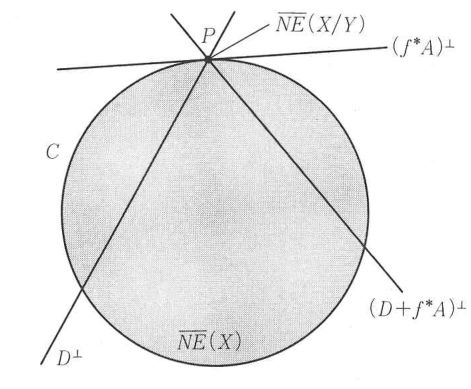
\includegraphics[width=0.60\textwidth]{figures/fig1.4.png}
\figtitle{1.4}{Abel 曲面示例中的曲线锥：圆 $C$ 为截口，点 $P$ 对应 $\overline{NE}(X/Y)$，三条直线为 $D^{\perp}$、$(f^*A)^{\perp}$、$(D+f^*A)^{\perp}$（原书 p.44）}
\end{figure}

% [原文 p.45]
使 $f$ 成为双有理的类似例子也可如下构成。设 $L$ 是 $E$ 上的丰富可逆层，$\pi:\PP_E(L\oplus\cO_E)\to E$ 是 $\PP^1$-丛，而 $g:\PP_E(L\oplus\cO_E)\to V$ 是 $\pi$ 的负截面 $S$ 的收缩。令
\[ h=id_E\times g:\ E\times\PP_E(L\oplus\cO_E)\to E\times V, \]
则 $h$ 是双有理映射，注意它在 $X\cong E\times S$ 上给出态射 $f$。此时 $G:=(id_E\times\pi)^*D$ 是 h-nef 的，但 $G+h^*B|_X=D+f^*(B|_E)$，故对任何 $B$，$G+h^*B$ 都不是 nef 的。
\end{example}

% [Tutor Note: 例 1.46 说明 f-nef 与 nef 的差别：$D$ 在每个纤维上次数为零（甚至数值平凡），却因纤维方向之外的相交形式为负，无论如何加 $f^*A$ 都无法变正。相对判别法必须用 $\overline{NE}(X/Y)$ 而非 $\overline{NE}(X)$，原因正在此。]

% [原文 p.46]
% [本页原书为空白页]

\chapterreview{本章从标准类 $K_X$ 的负性出发，建立起“负性迫使有理曲线存在”这一贯穿全书的原理。§1.1 处理 $-K_X$ 丰富（Fano）的情形：定理 1.2 与命题 1.3 用双有理映射的不定点造出有理曲线；定理 1.10 进一步给出过任意点的有理曲线，且其与 $-K_X$ 的次数不超过 $\dim X+1$；推论 1.4、推论 1.5 则表明，只要一个双有理映射有不定点，像中就必含有理曲线。例 1.8 提醒我们，这些结论对一般紧复流形并不成立，代数簇的假设不可或缺。§1.2 把假设减弱为某条曲线 $C'$ 满足 $-(C'\cdot K_X)>0$，定理 1.13 仍然给出有理曲线，并同时控制其 $K_X$-次数与 $H$-次数之比。

证明的主干是折弯引理（推论 1.7、引理 1.9）：先让曲线“固定一点而形变”，其退化分解为若干有理曲线之和，于是只要附点形变空间的维数足够大便能得到次数更低的曲线；维数估计 $\dim\ge-(C\cdot f^*K_X)+(1-g(C))\dim X$ 正是保证这一点的关键。为得到高次自同态，Kollár 把问题搬到正特征，利用 Frobenius 态射的 $m$ 次幂；generic flatness 使交点数与亏格不随 $p$ 变化，于是几乎所有素数上都能造出有理曲线，再由原理 1.11 回到特征 $0$。这一“正特征化”手法是本章最值得记住的技术：它把特征 $0$ 下的形变问题转化为特征 $p$ 下现成的自同态。

§1.3 把上述结果翻译成锥的语言：先在定义 1.16、定义 1.17 中把 $1$-循环的数值等价与 $\overline{NE}(X)$ 的闭包讲清楚，再由锥定理 1.24 断言 $\overline{NE}(X)$ 由 $K_X\ge0$ 的部分与可数条极射线生成；把边界微移到 $(K_X+\epsilon H)\ge0$ 后只剩有限条极射线（推论 1.19 的紧性）。极射线对应簇的收缩（定义 1.25），于是极小模型纲领的第一步——找 $K_X$-负的极射线并收缩——有了严格的几何基础；例 1.27 则说明射影性并非自动成立，收缩之后仍须检验。§1.4 在曲面上把这一步走到底：定理 1.28 列出三种收缩，反复收缩使 Picard 数下降，最终得到极小模型（定理 1.29、要约 1.31）；三维情形（定理 1.32）则出现例外型收缩与小收缩等新现象。

§1.5 转向丰富性判别法：Kleiman 判别法（定理 1.18）把丰富性化为 $\overline{NE}(X)$ 上的正性，中井--Moishezon 判别法（定理 1.37）则用 Noether 归纳把正性落到每个闭子概形上，其证明依赖 Riemann--Roch 的渐近展开与定理 1.38。命题 1.41 把消没定理沿纤维方向归纳，从而把判别法相对化；两者都有相对版（定理 1.42、定理 1.44），为后续章节处理纤维化与收缩作准备。例 1.46 提醒我们，f-nef 远比 nef 弱，相对判别法必须用 $\overline{NE}(X/Y)$ 而不能用 $\overline{NE}(X)$。

综观全章，有理曲线的存在性、曲线锥的结构与收缩的存在性是同一件事的三个侧面：负性造曲线，曲线造极射线，极射线造收缩。本章遗留的问题也很清楚：极射线是否总能收缩（例 1.27 给出反例），三维以上的收缩如何分类，以及奇点如何处理——这些正是第 3 章极小模型纲领的主题。}
